\documentclass[letterpaper]{amsart}
\usepackage{float}
\usepackage{times}
\usepackage{tikz}
\usepackage{calc}
\usepackage{booktabs, siunitx}
\usepackage{graphicx}
\usepackage{mathtools}
\usetikzlibrary{arrows.meta}

\title[Homework 2]{Homework 4 \\ OR647: Queueing Theory, Spring 2021}
\author{David Prentiss}
\email{dprentis@gmu.edu}
\date{\today}

\begin{document}
\maketitle

\section{Problem 3.32} %1
You are managing a call center where the arrival rate is 500 calls per hour
and the service time is exponential with a mean of 2 minutes.
\subsection*{a}
What is the approximate number of servers needed so that the probability that a
customer has a non-zero wait in queue is 10\%?

\subsubsection*{Solution}
Let $\lambda = \frac{500}{60}=\frac{25}{3}$, $\mu=\frac{1}{2}=0.5$, and $\alpha=0.10$. Then
$r=\frac{\lambda}{\mu}=\frac{50}{3}$, $\beta\approx1.420$ and
\begin{equation*}
  c\approx r + \beta\sqrt{r} = 22.465 \approx 23
\end{equation*}

\subsection*{b}
If the arrival rate increases by 60\%, what is the approximate number of
servers needed to maintain the same level of service?

\subsubsection*{Solution}
Let $\lambda = 1.6\cdot\frac{500}{60}=\frac{40}{3}$, $\mu=\frac{1}{2}=0.5$,
and $\beta\approx1.420$. Then $r=\frac{\lambda}{\mu}=\frac{80}{3}$ and
\begin{equation*}
  c\approx r + \beta\sqrt{r} = 34.000 \approx 34
\end{equation*}

\subsection*{c}
If the average time to complete a call increases by 1 minute (assuming
the original arrival rate of 500 calls per hour), what is the approximate
number of servers needed to maintain the same level of service?
\subsubsection*{Solution}
Let $\lambda = \frac{500}{60}=\frac{25}{3}$, $\mu=\frac{1}{3}$
and $\beta\approx1.420$. Then $r=\frac{\lambda}{\mu}=25$ and
\begin{equation*}
  c\approx r + \beta\sqrt{r} = 32.101 \approx 33
\end{equation*}

\subsection*{d}
For parts (a) and (b), compute the exact minimum number of servers
needed to achieve no more than 10\% probability of non-zero wait in
queue. Compute the exact expected wait in queue for the two scenarios.
Are they the same?
\subsubsection*{Solution}
For part (a) Let $r=\frac{\lambda}{\mu}=\frac{50}{3}$. Then $\rho=r/c = \frac{50}{3c}$.
The probability of nonzero wait time is given by
\begin{equation*}
  C(c,r)=\frac{r^c}{c!(1-\rho)}\left( \frac{r^c}{c!(1-\rho)}+\sum_{n=0}^{c-1}\frac{r^n}{n!}\right)^{-1}
\end{equation*}
Starting with our estimate, $c\approx23$, we have
\begin{align*}
  C(23,\frac{50}{3}) &= 0.101 > 0.10 \\
  C(24,\frac{50}{3}) &= 0.064 < 0.10\ \checkmark
\end{align*}

For part (b) Let $r=\frac{\lambda}{\mu}=\frac{80}{3}$ with $C(c,r)$ as before.
Starting with our estimate, $c\approx34$, we have
\begin{align*}
  C(34,\frac{80}{3}) &= 0.122 > 0.10 \\
  C(35,\frac{80}{3}) &= 0.085 < 0.10\ \checkmark
\end{align*}

\section{Problem 3.37} %10
You are managing a call center where arrivals follow a Poisson process with
rate of 300 calls per hour and the service time is exponential with a mean of
2 minutes.
\subsection*{a}
What is the approximate number of servers needed so that the probability that a
customer has a nonzero wait in queue is 5\%?

\subsubsection*{Solution}
Let $\lambda = \frac{300}{60}=5$, $\mu=\frac{1}{2}=0.5$, and $\alpha=0.05$. Then
$r=\frac{\lambda}{\mu}=10$, $\beta\approx1.740$ and
\begin{equation*}
  c\approx r + \beta\sqrt{r} = 15.502 \approx 16
\end{equation*}

\subsection*{b}
If the arrival rate doubles, what is the approximate number of servers
needed to maintain the same level of service?

\subsubsection*{Solution}
Let $\lambda = 2\cdot\frac{300}{60}=10$, $\mu=\frac{1}{2}=0.5$, and $\beta\approx1.740$. Then
$r=\frac{\lambda}{\mu}=20$ and
\begin{equation*}
  c\approx r + \beta\sqrt{r} = 27.781 \approx 28
\end{equation*}

\subsection*{c}
Suppose that you are given the steady-state probabilities $p_0,p_1,\ldots,p_n$.
Give a formula or procedure for computing the expected number of
customers in queue and the variance of the number of customers in
queue using these values.

\subsubsection*{Solution}
Given a sequence of $n+1$ steady-state probabilities with $n$ large enough that
$p_n \approx 0$, the average number in the queue, $L_q$, is approximated by the
sums of the length of the queue in each state weighted by the probability of its
respective probability or


\begin{equation*}
  L_q = \sum_{i=c+1}^n(i-c)p_i
\end{equation*}
where $c$ is the number of servers.
Here, $i-c$ serves as the size of the queue in each state $n$ and, we may ignore
$i\leq c$ since the length of the queue in those states is 0.
The variance then is
\begin{equation*}
  \sigma_{L_q}^2 = \sum_{i=c+1}^n(i-c-L_q)^2p_i
\end{equation*}
Care must be taken with an estimate such as this since the distribution of queue
lengths may be heavy-tailed.
As such, $n$ may need to be very large to avoid a significant estimation error.

\section{} %3
A call center has 400 service representatives. The offered load is 360. Assume the
call center can be modeled as an $M/M/c$ queue. The company believes that its
current level of service (as measured by the fraction of customers who
immediately connect to a representative) is good. However, demand has been
increasing, so the company decides to hire 50 more representatives. If demand
increases by 5\% every week, approximately how many weeks will it take before
the service level (with 450 representatives) drops below its current level (with 400
representatives).

\subsubsection*{Solution}

Let $r=\frac{\lambda}{\mu} = 360$ and $c=400$.
Then the level of service is
\begin{equation*}
  W_q(0) = 1-C(400,360)\approx 0.977.
\end{equation*}
Now let the offered load during week $n$ be $\{r_n\}=\{378, 396.9, 416.745, 437.582,
459.461\}$ and $c=450$.
Then the level of service during week in is $n$
\begin{equation*}
  \{W_q(0)_n\} = \{1-C(450,r_n)\}\approx
  \{1.000, 0.995, 0.931, 0.556, -0.663\}
\end{equation*}
From these results we see that the additional representatives maintain the
previous level of service for the first \emph{two weeks} of increasing demand.
Note also that the negative level of service in week five is meaningless since
during that week $r=459.461>c=450$.

\section{} %4
A company owns a group license for a particular optimization software package.
The license allows for $n$ employees to use the package simultaneously. When an
employee logs in to use the software, if $n$ people are currently using the package,
then the employee is denied access to the software. Requests for use of the
software follow a Poisson process, where the mean arrival rate (per hour) varies
by time of day, as shown in the graph below. The time a user spends using the
software is exponentially distributed with a mean of 30 minutes. The company
wants to buy enough licenses $n$ so that, during the busiest hour of the day, at least
95\% of people who log in to use the software are able to immediately use it. What
is the minimum number $n$ of licenses needed?

\subsubsection*{Solution}
Let $\lambda=8$, $\mu = \frac{1}{30}(60) = 2$.
Then $r = 4$.
By incrementing $n$ by one license and calculating the level of service $W_q(0)
= 1 - C(n,r)$ we find that \emph{9 licenses} are necessary to achieve a level of
service of 95\%.
We can begin with five licenses since queues are unstable where $c\leq r$.
\begin{table}[H]
  \label{tab:1}
  \begin{tabular}{cS}
    \toprule
    {$n$} & {$C(n,r)$} \\
    \midrule
    5& 0.446 \\
    6& 0.715 \\
    7& 0.865 \\
    8& 0.941 \\
    9& 0.976\ \checkmark \\
    \bottomrule
  \end{tabular}
\end{table}
\section{Problem 3.50} %5
Customers arrive to a sandwich shop according to a Poisson process with rate 10
per hour. Service times are exponential with rate 4 per hour. The shop has 2
servers. At most, the shop can hold 6 customers in the queue. Beyond that, the
line goes out the door. Thus, we assume that when there are 6 customers in the
queue, additional customers are turned away.
\subsection*{a}
Draw a rate transition diagram for this system.
\subsubsection*{Solution}
\begin{figure}[H]
  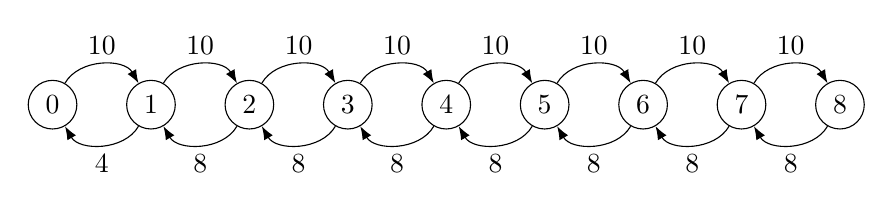
\begin{tikzpicture}[node distance={1.25cm}, state/.style = {draw, circle}]
    \node[state] (N) {0};
    \node[state] (A) [right of=N] {1};
    \node[state] (B) [right of=A] {2};
    \node[state] (C) [right of=B] {3};
    \node[state] (D) [right of=C] {4};
    \node[state] (E) [right of=D] {5};
    \node[state] (F) [right of=E] {6};
    \node[state] (G) [right of=F] {7};
    \node[state] (H) [right of=G] {8};

    \path[-Latex] (N) edge[bend left=60] node[above] {10} (A);
    \draw[-Latex] (A) edge[bend left=60] node[below] {4} (N);
    \path[-Latex] (A) edge[bend left=60] node[above] {10} (B);
    \draw[-Latex] (B) edge[bend left=60] node[below] {8} (A);
    \path[-Latex] (B) edge[bend left=60] node[above] {10} (C);
    \draw[-Latex] (C) edge[bend left=60] node[below] {8} (B);
    \path[-Latex] (C) edge[bend left=60] node[above] {10} (D);
    \draw[-Latex] (D) edge[bend left=60] node[below] {8} (C);
    \path[-Latex] (D) edge[bend left=60] node[above] {10} (E);
    \draw[-Latex] (E) edge[bend left=60] node[below] {8} (D);
    \path[-Latex] (E) edge[bend left=60] node[above] {10} (F);
    \draw[-Latex] (F) edge[bend left=60] node[below] {8} (E);
    \path[-Latex] (F) edge[bend left=60] node[above] {10} (G);
    \draw[-Latex] (G) edge[bend left=60] node[below] {8} (F);
    \path[-Latex] (G) edge[bend left=60] node[above] {10} (H);
    \draw[-Latex] (H) edge[bend left=60] node[below] {8} (G);
  \end{tikzpicture}
\end{figure}
\subsection*{b}
Determine the fraction of customers that are turned away.
\subsubsection*{Solution}
Let $\lambda = 10$, $\mu=4$, and $c=2$. Then $K=6+c=8$, $r=\lambda/\mu = 2.5$,
and $\rho=r/c=1.25$.

Customers are turned away whenever $N=K=8$. So, we need to find the probability
$p_8 = \text{Pr}[N=8]$.
First we use 3.48 for $\rho\neq 1$ to find the probability that there are zero customers in the
system,
$p_0\approx 0.0198$.
Then we use 3.47 for $n=K$ to find $p_8\approx 0.236$.
\subsection*{c}
If the arrival rate is very large, what is the approximate average wait in queue
(among customers who eventually complete service)?
\subsubsection*{Solution}
For $\rho\gg 1$, we assume a new customer always joins the queue when $N=7$.
In that case six customers must be served before the new customer is served. So
the wait time is
$\frac{1}{c\mu}(6)=\frac{6}{8}=0.75\text{\ hrs}$.
\section{Problem 3.55} %6
A cell tower can support $c$ simultaneous calls in its coverage area. Demand for
calls is Poisson with rate 30 per hour. Calls are exponential with a mean of 4
minutes. Calls are blocked when the cell tower is busy with $c$ calls in progress.
\subsection*{a}
If $c = 4$, determine the fraction of blocked calls.
\subsubsection*{Solution}
Let $\lambda=30$ and $\mu=\frac{1}{4}(60) = 15$.
Then $r=\frac{30}{15}=0.5$.
Calls are blocked when there are 4 calls in the system.
If we model the system as an $M/M/c/c$ queue, we can use Erlang-B to find
$\text{Pr}[N=c=4]=p_c\approx 0.0952$.
\subsection*{b}
Each completed call generates revenue of \$0.50. Each blocked call incurs a cost
of \$1.00. Which of the following cell towers has the shortest break-even time
(the time at which the cumulative revenue equals the cost of the cell tower): A
cell tower with $c = 2$, costing \$10,000; a cell tower with $c = 4$, costing
\$20,000; a cell tower with $c = 6$, costing \$30,000.
\subsubsection*{Solution}
Revenue per hour for such a cell tower is $\$0.50\lambda (1-p_c)$.
Likewise, the cost per hour is $\$1.00\lambda p_c$.
If $C_c$ is the one-time cost of commissioning a tower capable of $c$
simultaneous calls,
the break-even time, $t_c$ in hours is
\begin{equation*}
  t_c=
  \frac{
  C_c
}{
0.50\lambda (1-p_c) + 1.00\lambda p_c
}.
\end{equation*}
After converting to days we have
\begin{table}[H]
  \label{tab:1}
  \begin{tabular}{cSS}
    \toprule
    {$c$} &{$p_n$} & {$t_n$} \\
    \midrule
    2 &0.4 & 19.841\ \checkmark\\
4&0.095 & 50.725 \\
6&0.018 & 81.858 \\
    \bottomrule
  \end{tabular}
\end{table}
\section{} %7
Consider an $M/M/c/K$ queue with $\lambda = 20$, $\mu = 5$, $c = 4$, and $K = 7$
\subsection*{a}
For this system, find $p_n$ for $n = 0, 1, 2,\dots, 7$.
\subsubsection*{Solution}
Noting that $\rho = \frac{\lambda}{c\mu} = 1$,
Compute $p_0 = 0.0151$ using (3.48) for $\rho=1$.
Then use (3.47) to find
$p_1, p_2,\dots,p_7$.
\begin{table}[H]
  \label{tab:2}
  \begin{tabular}{cS}
    \toprule
    {$n$} & {$p_n$} \\
    \midrule
    0 & 0.0151 \\
    1 & 0.0603 \\
    2 & 0.1206 \\
    3 & 0.1608 \\
    4 & 0.1608 \\
    5 & 0.1608 \\
    6 & 0.1608 \\
    7 & 0.1608 \\
    \bottomrule
  \end{tabular}
\end{table}
\subsection*{b}
Find the probability that an arriving customer is able to enter service
immediately.
\subsubsection*{Solution}
The probability that a customer experiences no delay is the probability that
there are four our fewer customers, $N$, in the system. That is,
\begin{equation*}
  \text{Pr}[N\leq 4] = \sum_{n=0}^4 p_n = 0.518.
\end{equation*}

\subsection*{c}
Find the average number in queue $L_q$.
\subsubsection*{Solution}
\begin{equation*}
  L_q = \sum_{n=c+1}^K(n-c)p_n
  = 0.161\left[(5-4)+(6-4)+(7-4)\right]
  = 0.965
\end{equation*}
\subsection*{d}
Find the average waiting time in queue among customers who enter the
system.
\subsubsection*{Solution}
Let $\lambda_\text{eff} = \lambda(1-p_K) = 20(1-0.1608) = 16.7839$.
Then $W_q = L_q/\lambda_\text{eff} = 0.0575.$
\section{Problem 5.13} %8
The diagram below represents a model of a call center that sells tickets for a
local baseball team. Upon dialing, a customer first connects to an interactive
voice response (IVR) system (node A, ``If you would like to buy singlegame
tickets, press 1...''). There are two possible choices: (1) purchase
single-game tickets or (2) purchase multigame ticket packages. (Customers who do
not select any option effectively return to the IVR to start over.) Based on the
selection, the customer is then transferred to either the singlegame sales
representatives (node B) or the multigame sales representative (node C). After
selecting tickets, customers are transferred to another set of representatives
(node D) to handle credit card payments. (From nodes B and C, customers may also
choose to be transferred to the other set of agents to select more tickets
before paying.) There is 1 representative at node B, 1 at node C, and 1 at node
D. The IVR system can handle an arbitrarily large number of calls
simultaneously. The service rates at each node are $\mu_A = 120$ per hour, $\mu_B = 30$
per hour, $\mu_C = 10$ per hour, and $\mu_D = 30$ per hour. The arrival rate to the center
is $\gamma = 30$ calls per hour. Suppose that all of the assumptions of an open
Jackson network apply. The transition probabilities are shown in the diagram
(probabilities that do not sum to 1 indicate the possibility of abandonment).
\begin{figure}[H]
  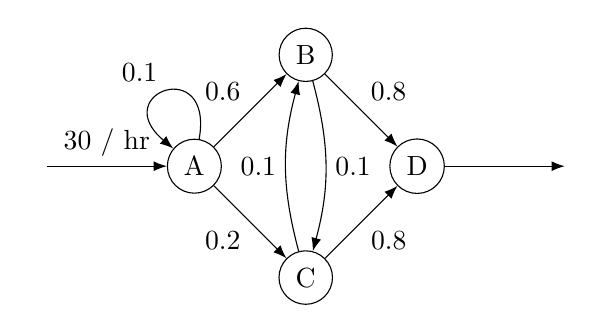
\begin{tikzpicture}[node distance={2cm}, state/.style = {draw, circle}]
    \node (I) {};
    \node[state] (A) [right of=I] {A};
    \node[state] (B) [above right of=A] {B};
    \node[state] (C) [below right of=A] {C};
    \node[state] (D) [below right of=B] {D};
    \node (O) [right of=D] {};


    \path[-Latex] (I) edge[] node[above] {30 / hr} (A);
    \path[-Latex] (A) edge[out=80, in=140, looseness=8] node[above left] {0.1} (A);
    \draw[-Latex] (A) edge[] node[above left] {0.6} (B);
    \draw[-Latex] (A) edge[] node[below left] {0.2} (C);
    \path[-Latex] (B) edge[bend left=15] node[right] {0.1} (C);
    \path[-Latex] (B) edge[] node[above right] {0.8} (D);
    \path[-Latex] (C) edge[bend left=15] node[left] {0.1} (B);
    \path[-Latex] (C) edge[] node[below right] {0.8} (D);
    \path[-Latex] (D) edge[] node[above] {} (O);
  \end{tikzpicture}
\end{figure}

\subsection*{a}
Calculate the average number of customers in the system.
\subsubsection*{Solution}
Let $\gamma_A=30$, $\gamma_B=\gamma_C=0$, $c_A = \infty$,
and $c_B=c_C=c_D=1$.
Then, solving the traffic equations, $\vec{\lambda}$ is
\begin{align*}
  \lambda_A &= 30 + 0.1\lambda_A = 33.333 \\ \\
  \lambda_B &= 0.6\lambda_A + 0.1\lambda_C=20.875 \\
  \lambda_C &= 0.2\lambda_A + 0.1\lambda_B=8.754 \\ \\
  \lambda_D &= 0.8\lambda_B + 0.8\lambda_C= 23.704
\end{align*}
So then $r_A= 33.333/120 = 0.278$,
$r_B= 20.875/30=0.696$,
$r_C= 8.754/10=0.875$,
and $r_D= 23.704/30=0.790$.

Modeling node A as $M/G/\infty$ we find $L_A=r_A=0.278$ and $L_q=W_q=0$.
For the remaining nodes we adopt the $M/M/1$ and calculate
$L_i=\frac{\lambda_i}{\mu_i-\lambda_i}$. Combining the results for all nodes we have
$\vec{L}=[0.278, 2.288, 7.027, 3.765]$ and
$L = 13.357$ customers.
\subsection*{b}
Calculate the average time a customer spends in the system.
\subsubsection*{Solution}
$W=\frac{L}{\gamma_A}=\frac{31.357}{30}\approx 0.445\text{ hr}\approx 26.7\text{ min}$.

\section{Problem 5.14} %9
For the open Jackson network shown below:
\begin{figure}[H]
  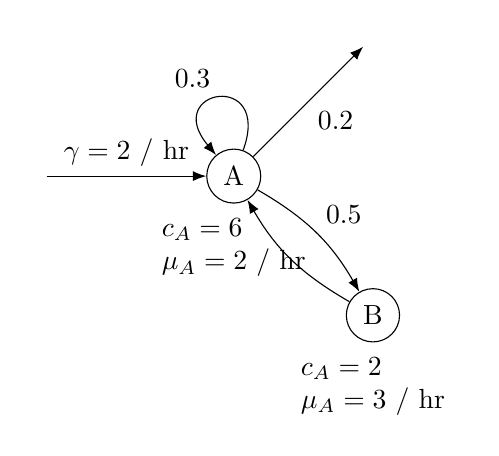
\begin{tikzpicture}[node distance={2.5cm}, state/.style = {draw, circle}]
    \node (I) {};
    \node[state] (A) [label=below:{\begin{tabular}{l}$c_A=6$\\ $\mu_A=2\text{ / hr}$\end{tabular}}] [right of=I] {A};
    %\node[state] (B) [label=below:{\begin{align*}c&=2\\ \mu&=3\text{/hr}\end{align*}}] [below right of=A] {B};
    \node[state] (B) [label=below:{\begin{tabular}{l}$c_A=2$\\ $\mu_A=3\text{ / hr}$\end{tabular}}] [below right of=A] {B};
    \node (O) [above right of=A] {};

    \path[-Latex] (I) edge[] node[above] {$\gamma=2\text{ / hr}$} (A);
    \path[-Latex] (A) edge[out=70, in=130, looseness=8] node[above left] {0.3} (A);
    \path[-Latex] (A) edge[bend left=15] node[above right] {0.5} (B);
    \path[-Latex] (B) edge[bend left=15] node[left] {} (A);
    \path[-Latex] (A) edge[] node[below right] {0.2} (O);
  \end{tikzpicture}
\end{figure}
\subsection*{a}

Determine the average wait in queue at each station
\subsubsection*{Solution}
Let $\gamma_B=0$.
Then, solving the traffic equations, $\vec{\lambda}$ is
\begin{align*}
  \lambda_A &= 2 + 0.3\lambda_A + \lambda_B = 10 \\
  \lambda_B &= 0.5\lambda_A=5
\end{align*}
\subsection*{b}
Determine the average time a customer spends in the overall system
(from arrival to exit from the system).
\subsubsection*{Solution}
By adopting the $M/M/c$ model we find $L_q$ and $L$ for each node.
That is, $L_{qA}\approx 2.938$,
$L_{qB}\approx 3.788$,
$L_{A}\approx 7.938$,
and $L_{B}\approx 5.454$.
Finally,
\begin{equation*}
  W=\frac{L_A+L_B}{\gamma}\approx 6.696\text{ hr}.
\end{equation*}

\subsection*{c}
Determine the rate that customers exit the system.
\subsubsection*{Solution}
Customers leave the system at $0.2\lambda_A=2/\text{hr}$.
\subsection*{d}
Determine the average total time a customer spends at station A from
arrival to exit from the system.
\subsubsection*{Solution}
$W_A=L_A/\lambda_A= 0.794\text{ hr}$. I think this really only tells us about
each time a customer is at A, not the total time spent at A.
Maybe it should be $W_A(1 + r_{AA} + r_{AB} + 2r_{AA}r_{AB} + \dots)$?


\section{} %10
Widgets arrive to a production facility according to a Poisson process with rate
$\gamma=10\text{ / hr}$. To complete production, a widget must be processed by
four machines (A, B, C, and D; each of the four stations has a single machine).
The processing time at each machine is exponential with rate $\mu_A = \mu_B =
15\text{ / hr}$ and $\mu_C = \mu_D = 12\text{ / hr}$. After being processed by
machine B, a widget is inspected: 10\% of widgets are discarded, 20\% must
complete re-work starting from machine A, and 70\% move on to machine C.
Similarly, widgets are inspected after processing by machine D: 20\% are
discarded, 10\% must complete re-work starting from machine C, 10\% must
complete re-work starting from machine A and 60\% are completed. The inspection
time is assumed to be instantaneous (no queues forms at the inspection station).

\subsection*{a}
a. What is the rate that widgets complete production (i.e., widgets completed per
time, not counting widgets that are discarded)?
\subsubsection*{Solution}
After solving the traffic equations,  we find
$\lambda_A=13.846$, $\lambda_B=13.846$, $\lambda_C=10.769$, and $\lambda_D=10.769$.
The rate that widgets complete production is 60\% of $\lambda_D$ or
$0.6\lambda_D = 6.462$ widgets per hour.

\subsection*{b}
b. What is the average number of widgets in the system?
\subsubsection*{Solution}
Let $c_A=c_B=c_C=c_d=1$. Then $r_A=13.846/15=0.923$, $r_B=13.846/15=0.923$,
$r_C=10.769/12=0.897$, and $r_D=10.769/12=0.897$. Calculating $L$ for $M/M/1$ we
have
\begin{equation*}
  L=\sum_{i\in{A,B,C,D}} \frac{r}{1-r} = 12 + 12 + 8.75 + 8.75 = 41.5\text{ widgets.}
\end{equation*}

\subsection*{c}
What is the average time a widget spends in the system?
\subsubsection*{Solution}
From Little's Law we have $W=L/\gamma=4.15$.
\end{document}